\newcommand{\installerTagResultsAucTable}{
    \begin{table}[H]
        \centering
        \begin{tabular}{|p{2,8cm}||P{2,4cm} P{2,4cm} P{2,4cm}|}
            \hline
            Installer Tag & ALOHA\newline (M/B only) & ALOHA & Proposed\newline Model \\
            \hline
            AUC-ROC & - & 0.971$\pm$0.004 & \textBF{0.981$\pm$0.000} \\
            \hline
        \end{tabular}
        \caption[Installer Tag prediction task AUC-ROC results]{AUC-ROC (Area Under Curve) of the different models for the \textbf{Installer Tag} prediction task. Results were aggregated over \textBF{2} training runs with different weight initializations and minibatch orderings. Best results are shown in \textbf{bold}.} \label{tab:installerTag_auc}
    \end{table}
}

\newcommand{\installerTagResultsAtFprTable}{
    \begin{center}
        \begin{longtable}[c]{|P{3,2cm}||P{1,8cm} P{1,8cm} P{1,8cm} P{1,8cm} P{1,8cm}|}
            \hline
            Installer Tag & \multicolumn{5}{c|}{{FPR}} \\
            & $10^{-5}$ & $10^{-4}$ & $10^{-3}$ & $10^{-2}$ & $10^{-1}$ \\
            \hline
            \endfirsthead

            \caption*{\raggedright ...continued from previous page} \\
            \hline
            Installer Tag & \multicolumn{5}{c|}{\textbf{FPR}} \\
            & $10^{-5}$ & $10^{-4}$ & $10^{-3}$ & $10^{-2}$ & $10^{-1}$ \\
            \hline
            \endhead

            \caption*{\raggedleft ...continued on next page} \\
            \endfoot

            \caption[Installer Tag prediction task results]{Mean and standard deviation results (TPR, Accuracy, Recall, Precision and F1-Score) of the different models for the \textbf{Installer Tag} prediction task at different \textbf{FPR}s (\textit{False Positive Rates}). Results were aggregated over \textBF{2} training runs with different weight initializations and minibatch orderings. Best results are shown in \textbf{bold}. Under \textbf{TPR} results are also presented the percentage reduction in mean detection error and in ROC curve standard deviation introduced by the \textit{Proposed Model} with respect to both \textit{ALOHA} model and \textit{Joint Embedding}.} \label{tab:installerTag_results_at_fpr} \\
            \endlastfoot

            \multicolumn{6}{|c|}{\textbf{TPR}} \\
            \hline
            ALOHA (M/B only) & - & - & - & - & - \\
            ALOHA & 0.202$\pm$0.004 & 0.288$\pm$0.021 & 0.431$\pm$0.075 & 0.724$\pm$0.044 & 0.908$\pm$0.019 \\
            Proposed Model & 0.220$\pm$0.010 & \textBF{0.340$\pm$0.020} & \textBF{0.515$\pm$0.028} & \textBF{0.773$\pm$0.009} & \textBF{0.951$\pm$0.007} \\
            \hline
            Error Reduction wrt\newline ALOHA (M/B only) & - & - & - & - & - \\
            Error Reduction wrt\newline ALOHA & 2.3\% & 7.3\% & 14.8\% & 17.8\% & 46.7\% \\
            \hline
            Std Reduction wrt\newline ALOHA (M/B only) & - & - & - & - & - \\
            Std Reduction wrt\newline ALOHA & -150.0\% & 4.8\% & 62.7\% & 79.5\% & 63.2\% \\
            \hline
            \multicolumn{6}{|c|}{\textbf{Accuracy}} \\
            \hline
            ALOHA (M/B only) & - & - & - & - & - \\
            ALOHA & 0.986$\pm$0.000 & 0.987$\pm$0.000 & 0.989$\pm$0.001 & 0.985$\pm$0.001 & 0.900$\pm$0.000 \\
            Proposed Model & 0.986$\pm$0.000 & \textBF{0.988$\pm$0.000} & \textBF{0.990$\pm$0.000} & \textBF{0.986$\pm$0.000} & \textBF{0.901$\pm$0.000} \\
            \hline
            \multicolumn{6}{|c|}{\textbf{Recall}} \\
            \hline
            ALOHA (M/B only) & - & - & - & - & - \\
            ALOHA & 0.202$\pm$0.004 & 0.288$\pm$0.021 & 0.431$\pm$0.075 & 0.724$\pm$0.044 & 0.908$\pm$0.019 \\
            Proposed Model & 0.220$\pm$0.010 & \textBF{0.340$\pm$0.020} & \textBF{0.515$\pm$0.028} & \textBF{0.773$\pm$0.009} & \textBF{0.951$\pm$0.007} \\
            \hline
            \multicolumn{6}{|c|}{\textbf{Precision}} \\
            \hline
            ALOHA (M/B only) & - & - & - & - & - \\
            ALOHA & 0.997$\pm$0.000 & 0.981$\pm$0.001 & 0.883$\pm$0.018 & 0.567$\pm$0.015 & 0.141$\pm$0.003 \\
            Proposed Model & \textBF{0.998$\pm$0.000} & \textBF{0.984$\pm$0.001} & \textBF{0.903$\pm$0.004} & \textBF{0.583$\pm$0.003} & \textBF{0.147$\pm$0.001} \\
            \hline
            \multicolumn{6}{|c|}{\textbf{F1 Score}} \\
            \hline
            ALOHA (M/B only) & - & - & - & - & - \\
            ALOHA & 0.337$\pm$0.006 & 0.445$\pm$0.025 & 0.576$\pm$0.072 & 0.636$\pm$0.026 & 0.244$\pm$0.004 \\
            Proposed Model & 0.360$\pm$0.014 & \textBF{0.505$\pm$0.022} & \textBF{0.656$\pm$0.024} & \textBF{0.665$\pm$0.005} & \textBF{0.254$\pm$0.002} \\
            \hline
        \end{longtable}
    \end{center}
}

\newcommand{\installerTagResultsSummaryTable}{
    \begin{table}[H]
        \centering
        \begin{tabular}{|P{3,2cm}||P{1,8cm} P{1,8cm} P{1,8cm} P{1,8cm} P{1,8cm}|}
            \hline
            \multicolumn{6}{|c|}{Installer Tag (at FPR $=1\%$)} \\
            \hline
            Model & TPR & Accuracy & Precision & Recall & F1 score \\
            \hline
            ALOHA (M/B only) & - & - & - & - & - \\
            ALOHA & 0.724$\pm$0.044 & 0.985$\pm$0.001 & 0.567$\pm$0.015 & 0.724$\pm$0.044 & 0.636$\pm$0.026 \\
            Proposed Model & \textBF{0.773$\pm$0.009} & \textBF{0.986$\pm$0.000} & \textBF{0.583$\pm$0.003} & \textBF{0.773$\pm$0.009} & \textBF{0.665$\pm$0.005} \\
            \hline
        \end{tabular}
        \caption[Summary of Installer Tag prediction task results]{Summary of the mean and standard deviation results of the different models for the \textbf{Installer Tag} prediction task at \textbf{FPR} $=1\%$. Results were aggregated over \textBF{2} training runs with different weight initializations and minibatch orderings. Best results are shown in \textbf{bold}.} \label{tab:installerTag_result_summary}
    \end{table}
}

\newcommand{\installerTagRocAlohaMB}{
    \begin{figure}[H]
        \vspace*{-0.5cm}
        \centering
        \includegraphics[width=0.6\textwidth]{./results/installer_tag_roc_alohaMB.png}
        \vspace*{-0.2cm}
        \caption[Installer Tag prediction task ALOHA (M/B only) ROC curve]{ROC curve and AUC statistics of \textBF{ALOHA (M/B only)} model for the \textbf{Installer Tag}. The line represents the \textit{mean} TPR at a given FPR, while the shaded region represents the \textit{standard deviation}. Statistics were computed over \textBF{2} training runs, each with random parameter initialization.}
        \label{fig:installerTagRocAlohaMB}
    \end{figure}
}

\newcommand{\installerTagRocAloha}{
    \begin{figure}[H]
        \vspace*{-0.5cm}
        \centering
        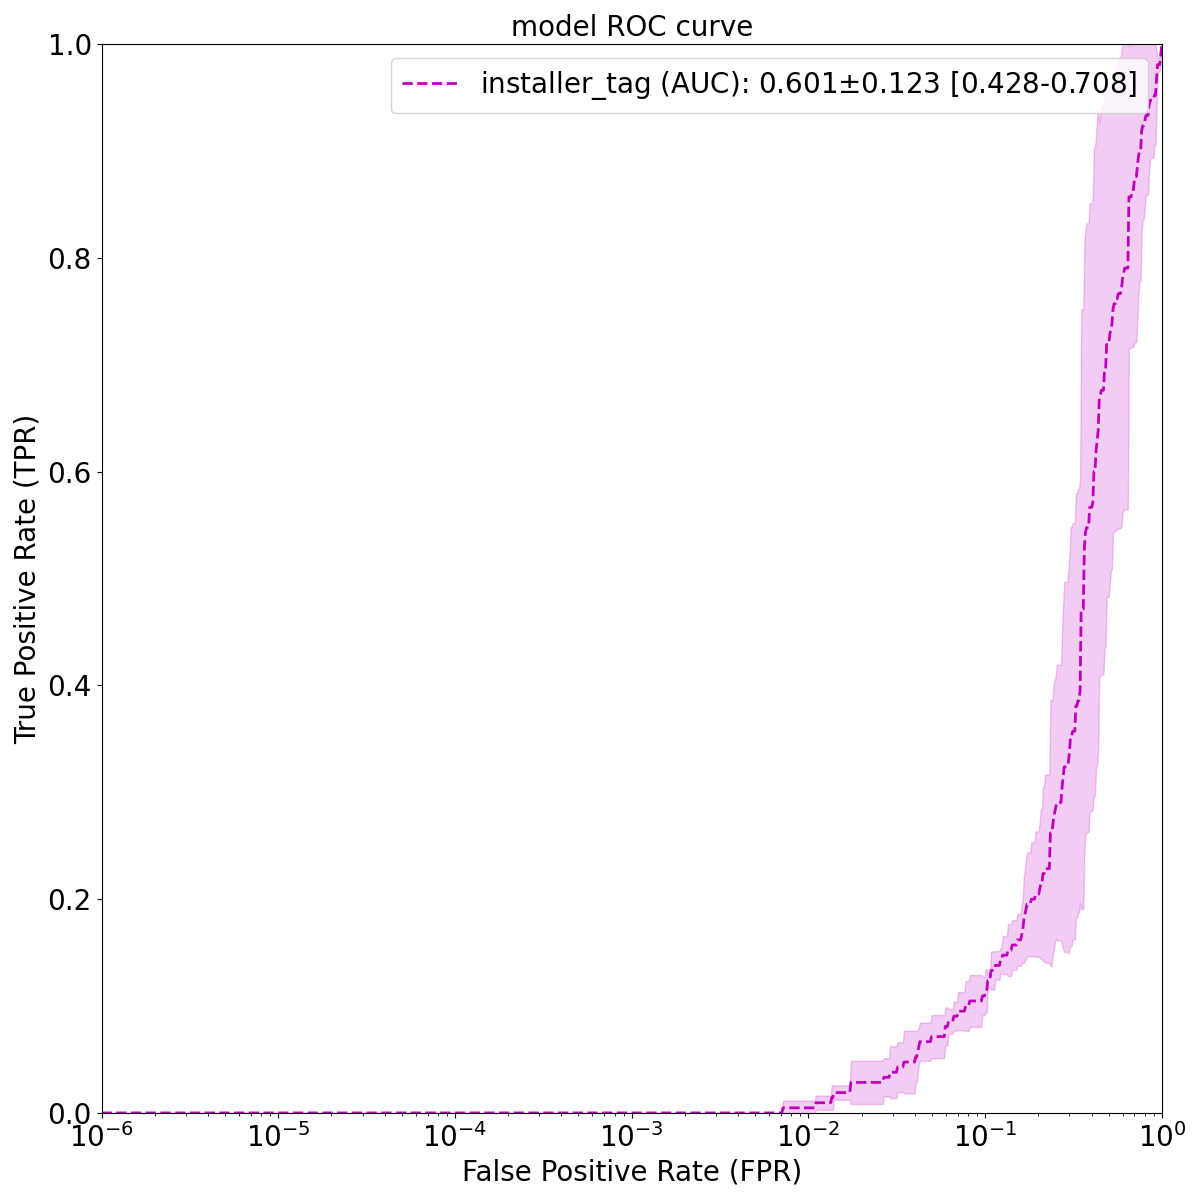
\includegraphics[width=0.6\textwidth]{./results/installer_tag_roc_aloha.png}
        \vspace*{-0.2cm}
        \caption[Installer Tag prediction task ALOHA ROC curve]{ROC curve and AUC statistics of \textBF{ALOHA} model for the \textbf{Installer Tag}. The line represents the \textit{mean} TPR at a given FPR, while the shaded region represents the \textit{standard deviation}. Statistics were computed over \textBF{2} training runs, each with random parameter initialization.}
        \label{fig:installerTagRocAloha}
    \end{figure}
}

\newcommand{\installerTagRocProposedMethod}{
    \begin{figure}[H]
        \vspace*{-0.5cm}
        \centering
        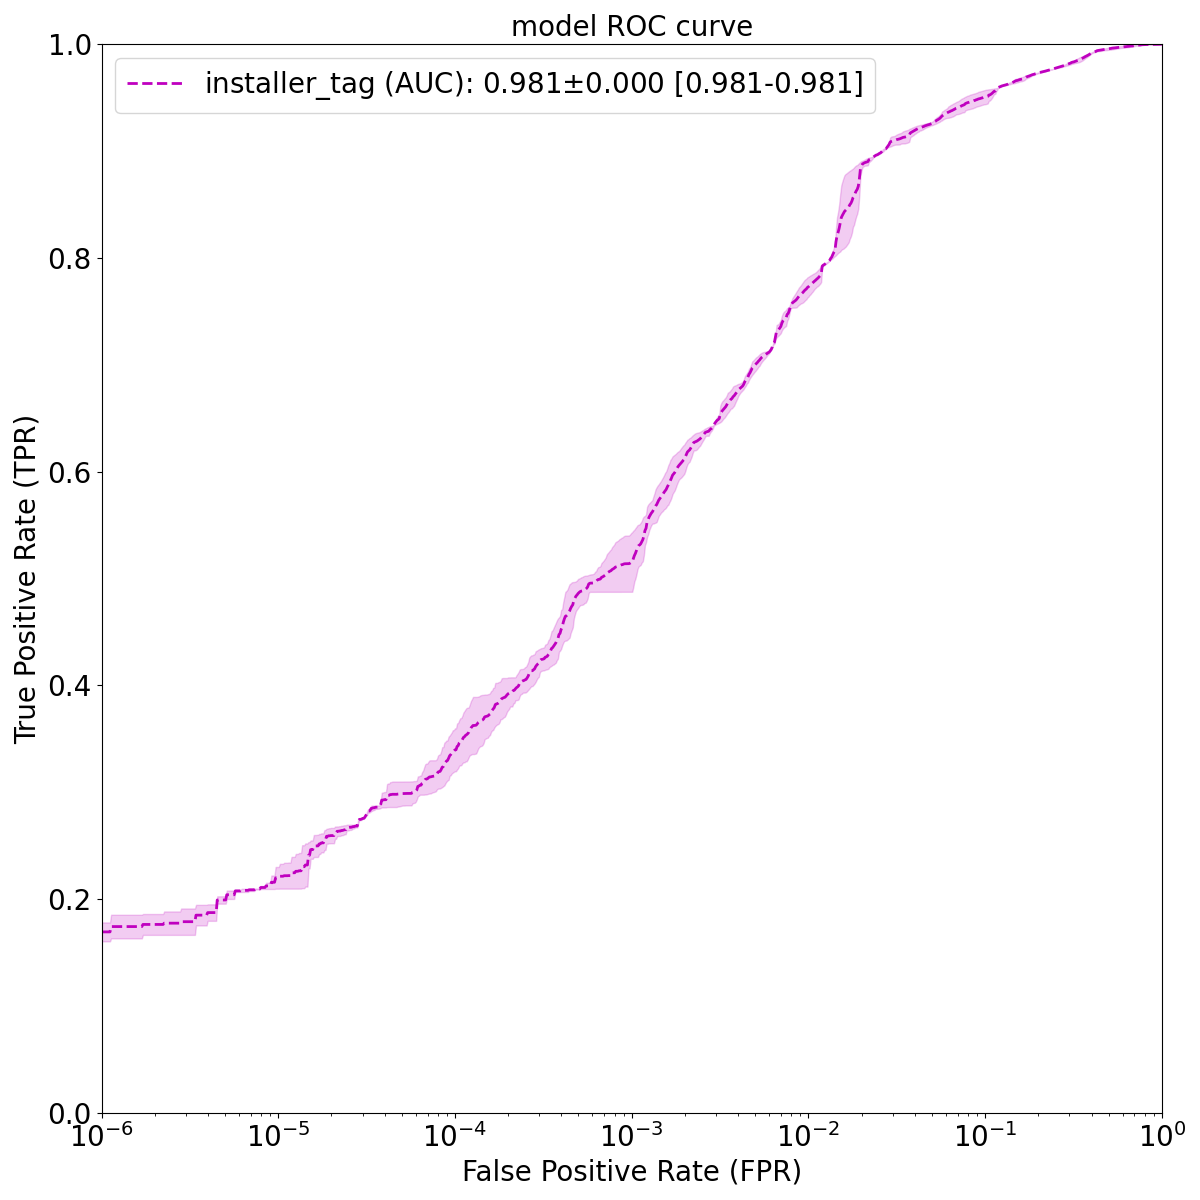
\includegraphics[width=0.6\textwidth]{./results/installer_tag_roc_proposedModel.png}
        \vspace*{-0.2cm}
        \caption[Installer Tag prediction task Proposed Model ROC curve]{ROC curve and AUC statistics of \textBF{Proposed Model} for the \textbf{Installer Tag}. The line represents the \textit{mean} TPR at a given FPR, while the shaded region represents the \textit{standard deviation}. Statistics were computed over \textBF{2} training runs, each with random parameter initialization.}
        \label{fig:installerTagRocProposedModel}
    \end{figure}
}
